\section{Background}
\label{sec:background}

%\todo{What should one understand in order to grasp this paper?}
Before we go into the algorithm, the following items must be explained. We
start with \emph{Markov decision processes (MDPs)}, then  discuss MCTS and
options and finally describe the \emph{video game description language (VGDL)}.

\subsection{Markov Decision Processes}
\label{subsec:mdps}
%\todo{MDPs}
In this paper, a game will be treated as an MDP, which is a
tuple $\langle S, A, T, R \rangle$. $S$ denotes the set of states. A state
contains all the information of the game's current condition: locations of
monsters, the avatar, etc. $A$ is a finite set of actions, the input an agent
can deliver to the game. $T$ a transition function defined as $T : S \times A
\times S \rightarrow \left[0,1\right]$. It defines the probabilities over the 
next states an agent can arrive in, when taking an action in a state.
$R$ is a reward function defined as $R: S \times A \times S \rightarrow
\mathbb{R}$. In this case, when the game score increases, only the increase is
seen as the reward. Algorithms typically maximize the cumulative reward, which
is analogous to the score. An MDP by definition has the \emph{Markov property},
which means that the conditional probability distribution of future states
depends only upon the present state. No information from previous states is
needed.

\todo{hoe relateren winnen en scores aan elkaar (maar misschien niet hier?)}

\subsection{Monte Carlo Tree Search}
\begin{figure}
	\centering
	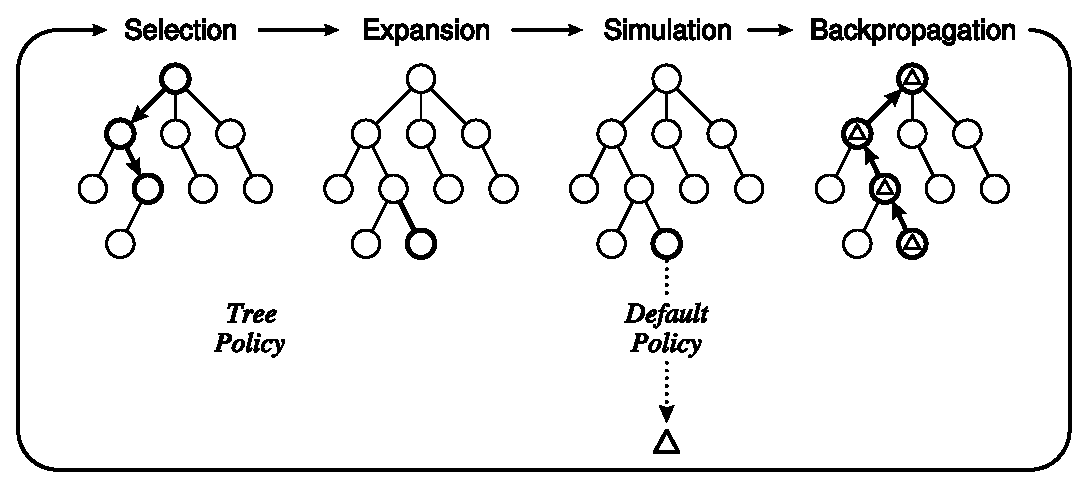
\epsfig{file=includes/mcts.eps, width=.6\columnwidth}
	\caption{One Monte Carlo tree search iteration}
	\label{fig:mcts}
\end{figure}

\label{subsec:mcts}
%\todo{MCTS}
The MCTS algorithm has been a core AI algorithm for a long time
\cite{browne2012survey}. It approximates the value of actions taken in a
specific state using the following method. A tree is built incrementally from
the states and actions that are visited in a game. Each node in the tree
represents a state, each connection in the tree represents an action taken in
that state leading to a state, which is represented by the next tree node. 
The process, as explained in figure \ref{fig:mcts} from \cite{browne2012survey},
consists of four phases that are constantly repeated. It
is started with the current game state, which is represented by the root node of
the tree. The first action is chosen by an \emph{expansion strategy} and
subsequently simulated, resulting in a new game state, for which a new node is
created. A \emph{rollout} is done from the new node, which means that a simulation is
run from the new node using a \emph{default policy} until a
predefined stop criterion is met or the game ends. A typical default policy
selects random actions. Finally, the score difference resulting from the rollout 
is backed up, or backpropagated, to the root node, which means that the reward
is saved to the visited nodes. Then a new iteration starts. When all actions are
expanded in the root node, we call that node \emph{fully expanded} and use a
\emph{selection strategy} to select a next node.  When a node is selected that
is not fully expanded, the expansion strategy is used to create a new
node, after which a rollout takes place, after which the results are backed up. 

	%\todo{Selection strategy}
	%(Term from pMCTS.pdf)
The selection strategy selects optimal actions in internal tree nodes, depending
on the values of the child nodes. An effective and very popular selection
strategy is the \emph{upper confidence tree (UCT)} \cite{kocsis2006bandit}, which balances the choice 
between poorly explored actions with a high uncertainty about their value and
actions that have been explored but have a higher value. A child node $j$ is
selected to maximise
\begin{equation}
	\label{eq:uct}
	UCT = 2C_p \sqrt{\frac{2 \ln n}{n_j}}
\end{equation}
Where $n$ is the number of times the current node has been visited, $n_j$ is the
number of times child $j$ has been visited and $C_p > 0$ is a constant , often
set to $\sqrt{2}$, that shifts priority from exploration to exploitation.
	
	%\todo{Expansion strategy}
In standard MCTS, each action is explored at least once in each node. After all
actions have been expanded, the node switches to the normal selection strategy
for exploration. Some variants reduce the branching factor of the tree by only
expanding the nodes selected by a special expansion strategy. A specific example
is the \emph{crazy stone} algorithm \cite{coulom2007efficient}, which is an
expansion strategy that was designed especially for Go. We will use this
strategy in the algorithm proposed in section \ref{sec:learning}.
When using crazy stone, an action $i$ is selected with a probability
proportional to $u_i$
\begin{equation}
	\label{eq:crazystone}
	u_i = \exp\left(K \frac{\mu_0 - \mu_i}{\sqrt{2\left(\sigma_0^2 +
\sigma_i^2\right)}}\right) + \epsilon_i
\end{equation}
Each action has an estimated value $\mu_i$ ordered in such a way that $\mu_0 >
\mu_1 > ... > \mu_N$, and a variance $\sigma_i^2$. $\epsilon_i$ prevents 
the probability of selecting a move to reach zero and its value is proportional to
the ordering of the expected values of the possible actions. K is a constant
that influences the exploration/exploitation trade off.
\begin{equation}
	\label{eq:epsilon}
	\epsilon_i = \frac{0.1 + 2^{-i} + a_i}{N}
\end{equation}
Where $a_i$ is 1 when an action is \emph{an atari move}, a go-specific
move that can otherwise easily be underestimated by MCTS.

	%\todo{Backup algorithm}
% TODO: Check if result and reward are used wrongly
After a rollout, the reward is backed up, which means that the estimated value
for every node that has been visited in this simulation is updated with the
reward of this simulation. Usually the estimated value of a node is the average
of all rewards backed up to that node.

\subsection{Options}
\label{subsec:options}
%\todo{Options}
For mimicking human game playing, defining and solving subgoals and subtasks, we
use options \cite{sutton1999between, barto2003recent}. An option is a predefined method of
reaching a specific subgoal. Formally, it is a triple $\langle I, \pi,
\beta\rangle$ in which $I \subseteq S$ is an initiation set, $\pi: S \times A
\rightarrow [0, 1]$ is a policy and $\beta: S^+ \rightarrow[0,1]$ is a
termination condition.

A policy $\pi$ defines the action that should be taken in a state. The
initiation set is a set of states in which the option can be started. When the
option starts, policy $\pi$ will be followed, until a state is reached that
satisfies a termination condition in $\beta$. Using options in an MDP removes
the Markov property for that process: the state information alone is no longer
enough to predict an agents actions, since the actions are now not only
state-dependant, also dependant on what option the agent has chosen in the past.
The process is now called a \emph{semi-Markov decision process (SMDP)}. For
convenience, we will call the original action set of the MDP $A$, and the set of
options $O$.  Normal actions can be treated as options as well. An option for
action $a$ has a initiation set $I = S$, the policy $\pi$ is taking action $a$
in all the states.  The termination condition is that action $a$ has been
performed once.

\subsection{Video Game Description Language}
\label{subsec:vgdl}
%\todo{Video Game Description Language}
This paper will use a framework called the video game description
language \cite{schaul2013video}, in which games can very easily be defined.

To define a game in VGDL, two files should be created. Firstly, the game
description should be made, which defines for each type of object what its
character in the level description is, what it looks like in the game, how it
interacts with other objects and the world, and when it disappears from the
game. Secondly, a level description should be made, in which each character maps
to an object in the game, on the same grid location as the character has in the
file. By only defining these two files a wide spectrum of games can be created.

The GVGAI competition uses a Java implementation of this framework and comes
with many games. The algorithm proposed in this paper will be benchmarked on
these games.
